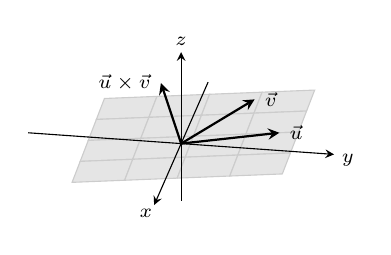
\begin{tikzpicture}
\begin{axis}%
[width=175pt,tick label style={font=\scriptsize},axis on top,
			axis lines=center,
			view={100}{40},
			name=myplot,
			xtick=\empty,
			ytick=\empty,
			ztick=\empty,
			ymin=-8,ymax=8,
			xmin=-10,xmax=10,
			zmin=-5, zmax=8,
			every axis x label/.style={at={(axis cs:\pgfkeysvalueof{/pgfplots/xmax},0,0)},xshift=-3pt,yshift=-3pt},
				xlabel={\scriptsize $x$},
			every axis y label/.style={at={(axis cs:0,\pgfkeysvalueof{/pgfplots/ymax},0)},xshift=5pt,yshift=-2pt},
				ylabel={\scriptsize $y$},
				every axis z label/.style={at={(axis cs:0,0,\pgfkeysvalueof{/pgfplots/zmax})},xshift=0pt,yshift=4pt},
				zlabel={\scriptsize $z$}
			]



\addplot3[domain=-7:5,y domain=-5:6,surf,faceted color=black!20,samples=5,black!10] {(-2*x+5*y)/27};

\draw[>=stealth,->,thick] (axis cs:0,0,0) -- (axis cs: -1,5,1) node [ right] {\scriptsize $\vec u$};

%\filldraw[black] (axis cs: 0,0,0.0) circle (1pt);

\draw[>=stealth,->,thick] (axis cs:0,0,0) -- (axis cs:-6,3,1) node [right] {\scriptsize $\vec v$};

\draw[>=stealth,->,thick] (axis cs:0,0,0) -- (axis cs: .4,-1,5.4) node [left ] {\scriptsize $\vec u\times \vec v$};



\end{axis}
%\node [right] at (myplot.right of origin)[shift={(-20pt,-8pt)}] {\scriptsize $y$};
%\node [above] at (myplot.above origin) [shift={(0,-5pt)}] {\scriptsize $z$};
\end{tikzpicture}









